% =====================================================================
%  PRESENTACIÓN OFICIAL EN LATEX BEAMER (16:9 WIDESCREEN)
%  TRABAJO PARCIAL --- ROBÓTICA Y SISTEMAS AUTÓNOMOS 2026-2
%  Robot Antropomórfico de 3 GDL (RRR)
%  Autores: Amit Roy Flores Rivera, Franklin Enrique Alegría Barboza,
%           José Luis Espinoza Chamaya, Raquel Medianero Huari,
%           Yasmín Mariela Urrego Montoya
%  Docente: Ing. Wilson Dennis Reyes Vásquez
%  UNI --- Facultad de Ingeniería Industrial y de Sistemas --- Posgrado
% =====================================================================
\documentclass[aspectratio=169,10pt,xcolor=table]{beamer}

% ---------- Codificación y fuentes ----------
\usepackage[utf8]{inputenc}
\usepackage[T1]{fontenc}
\usepackage{lmodern}
\usepackage{amsmath,amssymb,mathtools}
\usepackage{bm}
\usepackage{graphicx}
\usepackage{booktabs}
\usepackage{tabularx}
\usepackage{array}
\usepackage{multirow}
\usepackage{tcolorbox}
\tcbuselibrary{skins}
\usepackage{tikz}
\usetikzlibrary{arrows.meta,positioning,calc,shapes.geometric,fit,backgrounds}

% ---------- Paleta institucional UNI (idéntica al artículo) ----------
\definecolor{uniGranate}{HTML}{7A121C}
\definecolor{uniAzul}{HTML}{0B2447}
\definecolor{uniAzulC}{HTML}{1F6FEB}
\definecolor{uniRojo}{HTML}{B01818}
\definecolor{uniOro}{HTML}{C59B27}
\definecolor{cajaBg}{HTML}{F4F8FD}
\definecolor{cajaBorde}{HTML}{1F6FEB}
\definecolor{codigoBg}{HTML}{F4F6F9}
\definecolor{verdeOk}{HTML}{1B8E3A}
\definecolor{naranja}{HTML}{C97A0A}

% ---------- Configuración visual Beamer ----------
\usetheme{default}
\setbeamertemplate{navigation symbols}{}
\setbeamersize{text margin left=5.5mm, text margin right=5.5mm}
\setbeamercolor{background canvas}{bg=white}
\setbeamercolor{normal text}{fg=black!90}
\setbeamercolor{structure}{fg=uniAzul}
\setbeamercolor{itemize item}{fg=uniGranate}
\setbeamercolor{itemize subitem}{fg=uniAzulC}
\setbeamercolor{enumerate item}{fg=uniGranate}
\setbeamertemplate{itemize items}[circle]
\setbeamertemplate{enumerate items}[default]

% ---------- Espaciado compacto de ecuaciones para diapositivas ----------
\AtBeginDocument{%
  \setlength{\abovedisplayskip}{2.5pt}%
  \setlength{\belowdisplayskip}{2.5pt}%
  \setlength{\abovedisplayshortskip}{1.5pt}%
  \setlength{\belowdisplayshortskip}{1.5pt}%
}

% ---------- Encabezado institucional de doble línea sin desbordes ----------
\setbeamercolor{frametitle}{bg=uniAzul,fg=white}
\setbeamertemplate{frametitle}{%
  \nointerlineskip%
  \begin{beamercolorbox}[wd=\paperwidth,ht=8.4mm,dp=1.8mm,leftskip=5.5mm,rightskip=5.5mm]{frametitle}%
    \vbox to 8.0mm{\vfil%
      {\fontsize{10.2}{11.2}\selectfont\bfseries\color{white}\insertframetitle\par}%
      \vspace{0.5mm}%
      {\fontsize{7.0}{8.0}\selectfont\bfseries\color{uniOro!90!white}\insertframesubtitle\par}%
    \vfil}%
  \end{beamercolorbox}%
  \nointerlineskip%
  \hbox to \paperwidth{{\color{uniOro}\rule{\paperwidth}{0.55mm}}}%
  \vspace{-1.8mm}%
}

% ---------- Pie de página institucional en 1 sola línea ----------
\setbeamertemplate{footline}{%
  \leavevmode%
  \hbox{%
    \begin{beamercolorbox}[wd=0.24\paperwidth,ht=3.6mm,dp=1.1mm,leftskip=3.5mm]{foot1}%
      \color{white}\fontsize{5.6}{6.8}\selectfont\bfseries UNI \,---\, POSGRADO FIIS (2026-2)
    \end{beamercolorbox}%
    \begin{beamercolorbox}[wd=0.60\paperwidth,ht=3.6mm,dp=1.1mm,center]{foot2}%
      \color{white}\fontsize{5.6}{6.8}\selectfont Trabajo Parcial: Robot Antropomórfico RRR de 3\,GDL \,|\, Flores, Alegría, Espinoza, Medianero, Urrego
    \end{beamercolorbox}%
    \begin{beamercolorbox}[wd=0.16\paperwidth,ht=3.6mm,dp=1.1mm,rightskip=3.5mm,right]{foot3}%
      \color{uniOro}\fontsize{5.8}{6.8}\selectfont\bfseries Diapositiva \insertframenumber{} / \inserttotalframenumber
    \end{beamercolorbox}%
  }%
}
\setbeamercolor{foot1}{bg=uniGranate,fg=white}
\setbeamercolor{foot2}{bg=uniAzul,fg=white}
\setbeamercolor{foot3}{bg=uniAzul,fg=uniOro}

% ---------- Cajas tipo callout (indivisibles, idénticas al paper) ----------
\newtcolorbox{cajadef}[1][]{%
  enhanced,
  colback=cajaBg, colframe=cajaBorde,
  boxrule=0.55pt, arc=1.8pt,
  left=4.5pt, right=4.5pt, top=2.5pt, bottom=2.5pt,
  toptitle=1.8pt, bottomtitle=1.8pt,
  fonttitle=\fontsize{7.2}{8.5}\selectfont\bfseries\color{white},
  coltitle=white, colbacktitle=cajaBorde,
  title={#1}}

\newtcolorbox{cajaidea}[1][]{%
  enhanced,
  colback=green!5!white, colframe=verdeOk,
  boxrule=0.55pt, arc=1.8pt,
  left=4.5pt, right=4.5pt, top=2.5pt, bottom=2.5pt,
  toptitle=1.8pt, bottomtitle=1.8pt,
  fonttitle=\fontsize{7.2}{8.5}\selectfont\bfseries\color{white},
  coltitle=white, colbacktitle=verdeOk,
  title={#1}}

\newtcolorbox{cajaadv}[1][]{%
  enhanced,
  colback=orange!8!white, colframe=naranja,
  boxrule=0.55pt, arc=1.8pt,
  left=4.5pt, right=4.5pt, top=2.5pt, bottom=2.5pt,
  toptitle=1.8pt, bottomtitle=1.8pt,
  fonttitle=\fontsize{7.2}{8.5}\selectfont\bfseries\color{white},
  coltitle=white, colbacktitle=naranja,
  title={#1}}

% ---------- Comandos matemáticos abreviados ----------
\newcommand{\Real}{\mathbb{R}}
\newcommand{\T}{^{\!\top}}
\newcommand{\norm}[1]{\left\lVert#1\right\rVert}
\newcommand{\abs}[1]{\left\lvert#1\right\rvert}
\newcommand{\qdot}{\dot{\bm{q}}}
\newcommand{\qddot}{\ddot{\bm{q}}}
\newcommand{\pdot}{\dot{\bm{p}}}
\newcommand{\Jdls}{J^{\dagger}_{\text{\tiny DLS}}}

% ---------- Macros seguras para carga de imágenes en Overleaf y Local ----------
\newcommand{\LogoUNI}[1]{%
  \IfFileExists{logo.jpeg}{
\includegraphics[height=#1,keepaspectratio]{logo.jpeg}}{%
    \IfFileExists{logo_uni.png}{
\includegraphics[height=#1,keepaspectratio]{logo_uni.png}}{}}%
}
\newcommand{\FigEnceste}[1]{%
  \IfFileExists{results/figuras_examen_parcial/fig_objetivo_enceste.png}{%
    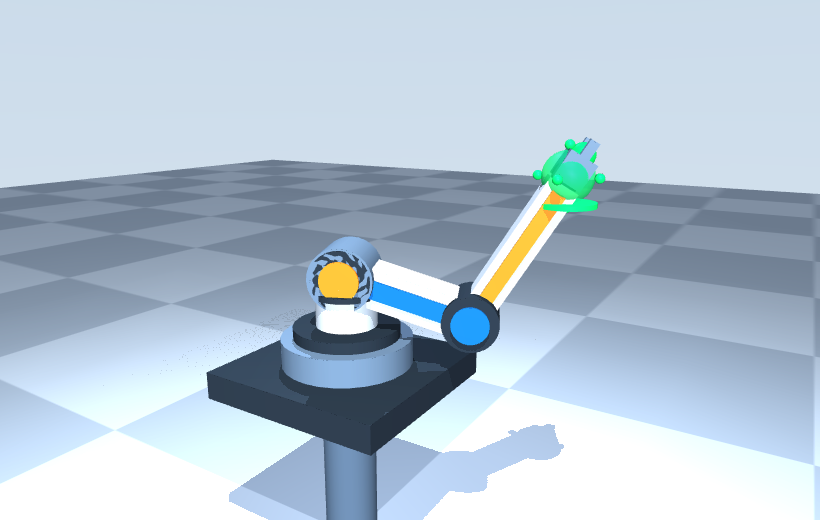
\includegraphics[width=#1,keepaspectratio]{results/figuras_examen_parcial/fig_objetivo_enceste.png}}{%
    \IfFileExists{results/figuras_examen_parcial/fig_objetivo_encestado_3d.png}{%
      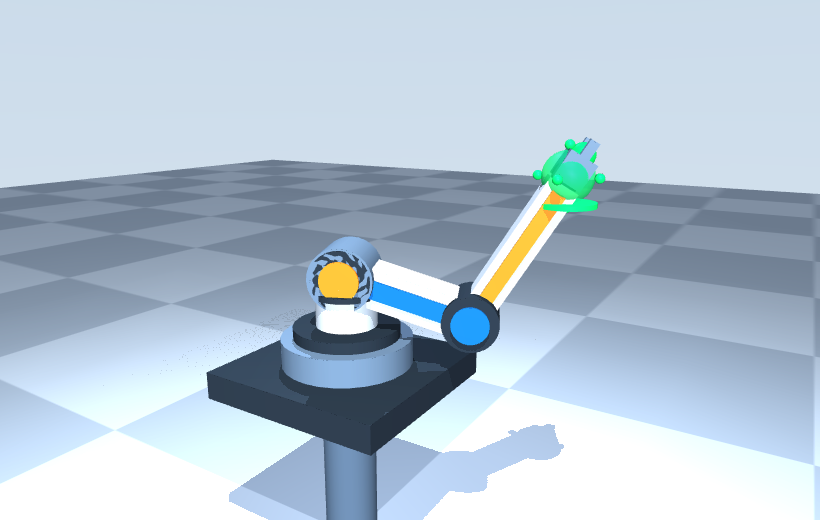
\includegraphics[width=#1,keepaspectratio]{results/figuras_examen_parcial/fig_objetivo_encestado_3d.png}}{}}%
}

% =====================================================================
\begin{document}

% =====================================================================
% DIAPOSITIVA 1: PORTADA INSTITUCIONAL UNI
% =====================================================================
{
\setbeamertemplate{footline}{}
\begin{frame}[plain]
\vspace{1.2mm}
\begin{columns}[T,totalwidth=\textwidth]
  % Columna izquierda: Escudo e Identidad Institucional
  \begin{column}{0.26\textwidth}
    \centering
    \vspace{1.0mm}
    \LogoUNI{2.55cm}\\[1.0mm]
    {\scriptsize\bfseries\scshape\color{uniGranate} Universidad Nacional\\de Ingeniería}\\[0.5mm]
    {\fontsize{5.6}{6.6}\selectfont\bfseries\color{uniAzul} Facultad de Ingeniería Industrial y de Sistemas --- Unidad de Posgrado}\\[1.2mm]
    \begin{tcolorbox}[enhanced,colback=uniAzul!6,colframe=uniAzul,boxrule=0.5pt,arc=2pt,left=3pt,right=3pt,top=1.6pt,bottom=1.6pt]
      \centering\fontsize{6.0}{7.2}\selectfont
      \textbf{\color{uniAzul}ASIGNATURA:}\\
      Robótica y Sistemas Autónomos\\[0.6mm]
      \textbf{\color{uniGranate}DOCENTE:}\\
      Ing.\ Wilson Dennis Reyes Vásquez\\[0.6mm]
      \textbf{\color{uniAzul}SEMESTRE:} 2026\,--\,2
    \end{tcolorbox}
  \end{column}

  % Columna derecha: Título del Trabajo Parcial y Equipo de Investigación
  \begin{column}{0.72\textwidth}
    \vspace{0.5mm}
    {\fontsize{6.6}{7.8}\selectfont\bfseries\color{uniGranate} MAESTRÍA EN INGENIERÍA DE SISTEMAS / INTELIGENCIA ARTIFICIAL}\\[0.4mm]
    {\color{uniAzul}\rule{\linewidth}{0.75pt}}\\[0.6mm]
    {\fontsize{12.2}{13.6}\selectfont\bfseries\color{uniAzul} «TRABAJO PARCIAL: ROBOT ANTROPOMÓRFICO DE 3\,GDL»}\\[0.6mm]
    {\fontsize{6.7}{7.9}\selectfont\bfseries\color{uniGranate} Modelado Cinemático (Geométrico, MTH y Denavit-Hartenberg), Cinemática Inversa de Doble Rama, Jacobiano Geométrico ($J_v, J_\omega$), Singularidades y Control Híbrido Evolutivo (CLIK-DLS / CTC / MPC / NSGA-II) en MATLAB y MuJoCo}\\[0.3mm]
    {\color{uniAzul}\rule{\linewidth}{0.75pt}}\\[0.5mm]

    \begin{cajadef}[Autores del Grupo de Investigación y Caso de Estudio]
      \fontsize{6.4}{7.6}\selectfont
      \begin{columns}[T,totalwidth=\linewidth]
        \begin{column}{0.51\linewidth}
          \begin{itemize}\setlength{\itemsep}{0pt}\setlength{\parskip}{0pt}
            \item \textbf{Flores Rivera, Amit Roy}
            \item \textbf{Alegría Barboza, Franklin Enrique}
            \item \textbf{Espinoza Chamaya, José Luis}
            \item \textbf{Medianero Huari, Raquel}
            \item \textbf{Urrego Montoya, Yasmín Mariela}
          \end{itemize}
        \end{column}
        \begin{column}{0.47\linewidth}
          \textbf{\color{uniAzul}Planta física de referencia:}\\
          Manipulador Antropomórfico RRR de 3\,GDL (Conejo Benítez, 2021)\\
          $d_1=0{,}079\;\text{m}$, $L_1=0{,}113\;\text{m}$, $L_2=0{,}140\;\text{m}$\\
          Alcance radial máx.: $R_{\max}=0{,}253\;\text{m}$
        \end{column}
      \end{columns}
    \end{cajadef}

    \vspace{0.3mm}
    \begin{cajaidea}[Entregables Verificados al 100\,\% según Rúbrica 2026-2]
      \fontsize{6.1}{7.2}\selectfont
      \textbf{1.} Triple derivación cinemática directa + verificación simbólica/numérica $\bullet$ \textbf{2.} IK analítica de doble rama ($\sigma=\pm 1$) con error $0{,}00\;\text{mm}$ $\bullet$ \textbf{3.} Jacobiano $6\times 3$ y mapa de Yoshikawa $w(\bm{q})$ $\bullet$ \textbf{4.} 5 leyes de control en MATLAB y Gemelo Digital 3D MuJoCo con modo juego «Circuito de 5 Aros».
    \end{cajaidea}
  \end{column}
\end{columns}

\begin{tikzpicture}[remember picture,overlay]
  \fill[uniGranate] (current page.north west) rectangle ([yshift=-2.4mm]current page.north east);
  \fill[uniOro] ([yshift=-2.4mm]current page.north west) rectangle ([yshift=-3.0mm]current page.north east);
  \fill[uniAzul] ([yshift=2.4mm]current page.south west) rectangle (current page.south east);
  \fill[uniOro] ([yshift=2.4mm]current page.south west) rectangle ([yshift=3.0mm]current page.south east);
\end{tikzpicture}
\end{frame}
}

% =====================================================================
% DIAPOSITIVA 2: CASO DE ESTUDIO REAL Y PARÁMETROS FÍSICOS
% =====================================================================
\begin{frame}{1. Introducción, Caso de Estudio Real y Arquitectura Funcional}{Manipulador Antropomórfico RRR de 3 GDL (Conejo Benítez, 2021)}
\begin{columns}[T,totalwidth=\textwidth]
  \begin{column}{0.56\textwidth}
    \begin{cajadef}[Planta Física Real: Brazo Antropomórfico RRR de 3\,GDL]
      \fontsize{6.8}{8.2}\selectfont
      Manipulador espacial rotacional (\textbf{R--R--R}) accionado por servomotores \textbf{Dynamixel} (Conejo Benítez, 2021, Tabla 3.2):\\[1mm]
      \resizebox{\linewidth}{!}{%
      \setlength{\tabcolsep}{3.5pt}
      \begin{tabular}{lccccc}
        \toprule
        \textbf{Articulación} & \textbf{Motor} & \textbf{Longitud} & \textbf{Rango [rad]} & $\bm{\tau}_{\max}$ & \textbf{Eje} \\
        \midrule
        $q_1$ (Cintura) & AX-18A & $d_1=0{,}079\;\text{m}$ & $[-2{,}80,\,+2{,}80]$ & $0{,}70\;\text{N\,m}$ & $Z_0$ vert. \\
        $q_2$ (Hombro)  & AX-12A & $L_1=0{,}113\;\text{m}$ & $[-1{,}25,\,+1{,}35]$ & $0{,}70\;\text{N\,m}$ & $Z_1$ horiz. \\
        $q_3$ (Codo)    & AX-12A & $L_2=0{,}140\;\text{m}$ & $[-2{,}40,\,+2{,}40]$ & $0{,}45\;\text{N\,m}$ & $Z_2\parallel Z_1$ \\
        \bottomrule
      \end{tabular}}
    \end{cajadef}

    \vspace{0.5mm}
    \begin{cajaidea}[Interrogantes Científicas y Aplicación Funcional]
      \fontsize{6.2}{7.3}\selectfont
      \begin{enumerate}\setlength{\itemsep}{0.4pt}
        \item \textbf{Equivalencia Cinemática:} ¿Cómo articular y comprobar simbólicamente los 3 métodos de cinemática directa (Geométrico, MTH y DH) junto con las 2 ramas de cinemática inversa?
        \item \textbf{Singularidades y DLS:} ¿Cómo caracterizar el Jacobiano $6\times 3$ y cruzar la frontera singular $\det J_v=0$ sin divergencia ($\norm{\qdot}\to\infty$)?
        \item \textbf{Control Óptimo y Modo Juego:} Un robot RRR de 3\,GDL controla $\bm{p}=[x,y,z]\T\in\Real^3$ ($R_{\max}=0{,}253\;\text{m}$), habilitando \textbf{Lente/Puntero Óptico ($<2{,}0\;\text{mm}$)} y \textbf{Circuito de 5 Aros} con cambio de estado visual 3D.
      \end{enumerate}
    \end{cajaidea}
  \end{column}

  \begin{column}{0.42\textwidth}
    \begin{cajadef}[Gemelo Digital 3D en MuJoCo (\texttt{main.py})]
      \centering
      \FigEnceste{0.84\linewidth}\\[0.8mm]
      {\fontsize{6.1}{7.3}\selectfont\color{uniAzul}
      \textbf{Figura 1.} Escena 3D interactiva en MuJoCo: esfera energética (\texttt{bola\_efector}) e inserción directa sobre aro objetivo (\texttt{objetivo\_aro\_base}) con conmutación a color \textbf{\color{verdeOk}Verde Esmeralda} al lograr $\norm{\bm{p}(t)-\bm{p}_{\text{obj}}}<2{,}0\;\text{mm}$.}
    \end{cajadef}
  \end{column}
\end{columns}
\end{frame}

% =====================================================================
% DIAPOSITIVA 3: CINEMÁTICA DIRECTA (MÉTODO 1: DENAVIT-HARTENBERG)
% =====================================================================
\begin{frame}{2. Cinemática Directa --- Método 1: Algoritmo de Denavit-Hartenberg}{Asignación de Marcos Ortonormales $\{S_0\}\dots\{S_3\}$ y Matrices Elementales $A_i$}
\begin{columns}[T,totalwidth=\textwidth]
  \begin{column}{0.45\textwidth}
    \begin{cajadef}[Esquema Cinemático 3D del Robot RRR]
      \centering
      \resizebox{0.97\linewidth}{!}{%
      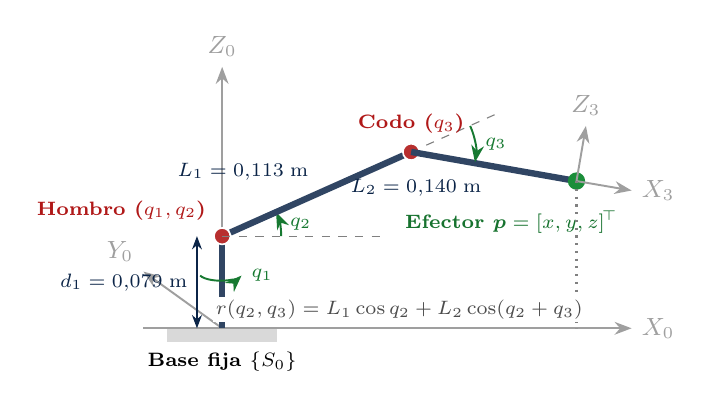
\begin{tikzpicture}[>=Stealth, font=\small,
         link/.style={line width=2.3pt, draw=uniAzul!85},
         joint/.style={circle, fill=uniRojo!90, draw=white, line width=0.6pt, inner sep=2.1pt},
         axis/.style={->, line width=0.7pt, color=gray!75},
         ang/.style={->, line width=0.7pt, color=verdeOk!85!black}]
        \fill[gray!30] (-0.7,0) rectangle (0.7,0.18);
        \draw[thick, uniAzul] (-0.7,0.18) -- (0.7,0.18);
        \node[below, font=\scriptsize\bfseries] at (0,0) {Base fija $\{S_0\}$};
        \draw[axis] (-1.0,0.18) -- (5.2,0.18) node[right] {$X_0$};
        \draw[axis] (0,0.18) -- (-1.0,0.90) node[above left] {$Y_0$};
        \draw[axis] (0,0.18) -- (0,3.5) node[above] {$Z_0$};
        \draw[link] (0,0.18) -- (0,1.35);
        \draw[<->, thin, color=uniAzul] (-0.32,0.18) -- (-0.32,1.35) node[midway, left, font=\scriptsize] {$d_1=0{,}079\;\text{m}$};
        \draw[ang] (-0.28,0.85) arc[start angle=200, end angle=340, x radius=0.28, y radius=0.10] node[right, font=\scriptsize] {$q_1$};
        \node[joint, label={[font=\scriptsize\bfseries, color=uniRojo]above left:{Hombro ($q_1,q_2$)}}] (sh) at (0,1.35) {};
        \draw[dashed, gray] (0,1.35) -- (2.1,1.35);
        \draw[ang] (0.75,1.35) arc[start angle=0, end angle=24, radius=0.75] node[midway, right, font=\scriptsize] {$q_2$};
        \coordinate (el) at (2.4,2.42);
        \draw[link] (sh) -- (el) node[midway, above left, font=\scriptsize, color=uniAzul] {$L_1=0{,}113\;\text{m}$};
        \draw[dashed, gray] (el) -- ($(el)+(1.1,0.49)$);
        \node[joint, label={[font=\scriptsize\bfseries, color=uniRojo]above:{Codo ($q_3$)}}] at (el) {};
        \coordinate (ef) at (4.5,2.05);
        \draw[link] (el) -- (ef) node[midway, below left, font=\scriptsize, color=uniAzul] {$L_2=0{,}140\;\text{m}$};
        \draw[ang] ($(el)+(0.75,0.33)$) arc[start angle=24, end angle=-9, radius=0.82] node[midway, right, font=\scriptsize] {$q_3$};
        \fill[verdeOk] (ef) circle (0.11);
        \draw[axis] (ef) -- ($(ef)+(0.70,-0.12)$) node[right] {$X_3$};
        \draw[axis] (ef) -- ($(ef)+(0.12,0.70)$) node[above] {$Z_3$};
        \node[below left, font=\scriptsize\bfseries, color=verdeOk!80!black] at ($(ef)+(0.65,-0.25)$) {Efector $\bm{p}=[x,y,z]\T$};
        \draw[dotted, thick, gray] (ef) -- (4.5,0.18);
        \draw[<->, thin, color=gray!60!black] (0,0.42) -- (4.5,0.42) node[midway, fill=white, inner sep=1pt, font=\scriptsize] {$r(q_2,q_3) = L_1\cos q_2 + L_2\cos(q_2+q_3)$};
      \end{tikzpicture}}
    \end{cajadef}
  \end{column}

  \begin{column}{0.53\textwidth}
    \begin{cajadef}[Tabla 1. Parámetros de Denavit-Hartenberg Estándar]
      \centering
      \resizebox{\linewidth}{!}{%
      \setlength{\tabcolsep}{4pt}
      \begin{tabular}{cccccc}
        \toprule
        \textbf{Eslabón $i$} & $\theta_i$ (rad) & $d_i$ (m) & $a_i$ (m) & $\alpha_i$ (rad) & \textbf{Articulación} \\
        \midrule
        1 & $q_1$ & $d_1=0{,}079$ & $0{,}000$       & $+\pi/2$ & Rot. ($Z_0$ vert.) \\
        2 & $q_2$ & $0{,}000$     & $L_1=0{,}113$   & $0$      & Rot. ($Z_1$ horiz.) \\
        3 & $q_3$ & $0{,}000$     & $L_2=0{,}140$   & $0$      & Rot. ($Z_2\parallel Z_1$) \\
        \bottomrule
      \end{tabular}}
    \end{cajadef}

    \vspace{0.8mm}
    \begin{cajaidea}[Matrices Homogéneas Elementales (\texttt{DHL(theta,d,a,alpha)})]
      \fontsize{6.6}{8.0}\selectfont
      Cada transformación $A_i = \operatorname{Rot}_z(\theta_i)\operatorname{Trans}(a_i,0,d_i)\operatorname{Rot}_x(\alpha_i)$ resulta en:\\[1.2mm]
      \resizebox{\linewidth}{!}{$
      \setlength{\arraycolsep}{2.2pt}
      A_1=
      \begin{bmatrix}
      c_1 & 0 &  s_1 & 0\\
      s_1 & 0 & -c_1 & 0\\
      0   & 1 &  0   & d_1\\
      0   & 0   & 0 & 1
      \end{bmatrix},\;
      A_2=
      \begin{bmatrix}
      c_2 & -s_2 & 0 & L_1 c_2\\
      s_2 &  c_2 & 0 & L_1 s_2\\
      0   &  0   & 1 & 0\\
      0   &  0   & 0 & 1
      \end{bmatrix},\;
      A_3=
      \begin{bmatrix}
      c_3 & -s_3 & 0 & L_2 c_3\\
      s_3 &  c_3 & 0 & L_2 s_3\\
      0   &  0   & 1 & 0\\
      0   &  0   & 0 & 1
      \end{bmatrix}
      $}\\[1.2mm]
      donde $c_i=\cos q_i$, $s_i=\sin q_i$. Producto acumulado: $T_0^3(\bm{q}) = A_1(q_1)A_2(q_2)A_3(q_3)$.
    \end{cajaidea}
  \end{column}
\end{columns}
\end{frame}

% =====================================================================
% DIAPOSITIVA 4: CINEMÁTICA DIRECTA (MTH Y GEOMÉTRICO + VERIFICACIÓN)
% =====================================================================
\begin{frame}{3. Cinemática Directa --- Métodos MTH, Geométrico y Verificación}{Equivalencia Exacta de los 3 Métodos en la Postura Inicial $\bm{q}_0=[-1{,}10,\;0{,}85,\;-0{,}75]\T\;\text{rad}$}
\begin{columns}[T,totalwidth=\textwidth]
  \begin{column}{0.51\textwidth}
    \begin{cajadef}[Matriz de Transformación Total $T_0^3(\bm{q}) = A_1 A_2 A_3$]
      \fontsize{6.5}{7.9}\selectfont
      Con $c_{23}=\cos(q_2+q_3)$ y $s_{23}=\sin(q_2+q_3)$:\\[1mm]
      \resizebox{0.96\linewidth}{!}{$
      \setlength{\arraycolsep}{2.5pt}
      T_0^3(\bm{q})=
      \begin{bmatrix}
      c_1 c_{23} & -c_1 s_{23} &  s_1 & (L_1 c_2 + L_2 c_{23})\,c_1\\
      s_1 c_{23} & -s_1 s_{23} & -c_1 & (L_1 c_2 + L_2 c_{23})\,s_1\\
      s_{23}     &  c_{23}     &  0   & d_1 + L_1 s_2 + L_2 s_{23}\\
      0          &  0          &  0   & 1
      \end{bmatrix}
      $}
    \end{cajadef}

    \vspace{0.7mm}
    \begin{cajaidea}[Método 2 (MTH Sucesivas) y Método 3 (Geométrico)]
      \fontsize{6.5}{7.9}\selectfont
      \begin{itemize}\setlength{\itemsep}{1pt}
        \item \textbf{MTH Sucesivas:} Composición espacial directa:\\[0.8mm]
        \resizebox{\linewidth}{!}{$
        T_0^3(\bm{q}) = \operatorname{Trans}_z(d_1)\operatorname{Rot}_z(q_1)\operatorname{Rot}_y(-q_2)\operatorname{Trans}_x(L_1)\operatorname{Rot}_y(-q_3)\operatorname{Trans}_x(L_2)
        $}
        \item \textbf{Método Geométrico Directo:} Proyección en el plano rotado $q_1$:
        \[
        \begin{cases}
        r(q_2,q_3) = L_1\cos q_2 + L_2\cos(q_2+q_3)\\
        x = r(q_2,q_3)\cos q_1,\quad y = r(q_2,q_3)\sin q_1,\quad z = d_1 + L_1\sin q_2 + L_2\sin(q_2+q_3)
        \end{cases}
        \]
      \end{itemize}
    \end{cajaidea}
  \end{column}

  \begin{column}{0.47\textwidth}
    \begin{cajadef}[Verificación Simbólica y Numérica de $T_0^1, T_0^2, T_0^3$]
      \fontsize{6.5}{7.9}\selectfont
      Evaluación en la postura inicial $\bm{q}_0=[-1{,}10,\;0{,}85,\;-0{,}75]\T\;\text{rad}$:\\[1mm]
      \resizebox{\linewidth}{!}{%
      \setlength{\tabcolsep}{2.5pt}
      \begin{tabular}{lll}
        \toprule
        \textbf{Matriz} & \textbf{Columna de posición $\bm{p}_i(\bm{q})$} & \textbf{Valor en $\bm{q}_0$ [m]} \\
        \midrule
        $T_0^1(1:3,4)$ & $[0,\;0,\;d_1]\T$ & $[0{,}0000,\;0{,}0000,\;0{,}0790]\T$ \\[1.2mm]
        $T_0^2(1:3,4)$ & $\begin{bmatrix}L_1 c_2 c_1\\ L_1 c_2 s_1\\ d_1+L_1 s_2\end{bmatrix}$ & $\begin{bmatrix}\phantom{-}0{,}033828\\ -0{,}066465\\ \phantom{-}0{,}163895\end{bmatrix}$ \\[4.2mm]
        $T_0^3(1:3,4)$ & $\begin{bmatrix}(L_1 c_2+L_2 c_{23})c_1\\ (L_1 c_2+L_2 c_{23})s_1\\ d_1+L_1 s_2+L_2 s_{23}\end{bmatrix}$ & $\begin{bmatrix}\phantom{-}0{,}097015\\ -0{,}190610\\ \phantom{-}0{,}177871\end{bmatrix}$ \\
        \bottomrule
      \end{tabular}}
    \end{cajadef}

    \vspace{0.7mm}
    \begin{cajaadv}[Consistencia Triple MATLAB $\leftrightarrow$ Python/MuJoCo]
      \fontsize{6.4}{7.8}\selectfont
      La discrepancia entre la cinemática simbólica MATLAB (\texttt{subs(T03)}), el método geométrico y el sensor \texttt{site\_xpos} de MuJoCo es $<10^{-15}\;\text{m}$.
    \end{cajaadv}
  \end{column}
\end{columns}
\end{frame}

% =====================================================================
% DIAPOSITIVA 5: CINEMÁTICA INVERSA DE DOBLE RAMA
% =====================================================================
\begin{frame}{4. Cinemática Inversa Analítica Cerrada de Doble Rama}{Resolución Exacta para Codo Abajo ($\sigma=+1$) y Codo Arriba ($\sigma=-1$)}
\begin{columns}[T,totalwidth=\textwidth]
  \begin{column}{0.52\textwidth}
    \begin{cajadef}[Derivación Geométrica-Algebraica en 3 Pasos]
      \fontsize{6.7}{8.1}\selectfont
      Dado el objetivo $\bm{p}_{\text{obj}}=[x,\,y,\,z]\T\in\Real^3$ dentro del volumen de trabajo:
      \begin{enumerate}\setlength{\itemsep}{1.5pt}
        \item \textbf{Acimut de cintura $q_1$ y desacople cilíndrico:}
        \[
        q_1 = \operatorname{atan2}(y,\,x),\quad r=\sqrt{x^2+y^2},\quad z'=z-d_1
        \]
        \item \textbf{Ángulo de codo $q_3^{(\sigma)}$ por Ley de Cosenos ($\sigma\in\{+1,-1\}$):}\\[1mm]
        \resizebox{\linewidth}{!}{$
        \cos q_3 = \dfrac{r^2+(z')^2 - L_1^2 - L_2^2}{2L_1 L_2}\in[-1,1],\quad
        q_3^{(\sigma)} = \operatorname{atan2}\!\Bigl(\sigma\sqrt{1-\cos^2 q_3},\,\cos q_3\Bigr)
        $}
        \item \textbf{Ángulo de hombro $q_2^{(\sigma)}$ por descomposición trigonométrica:}\\[1mm]
        \resizebox{\linewidth}{!}{$
        k_1 = L_1+L_2\cos q_3^{(\sigma)},\;\; k_2 = L_2\sin q_3^{(\sigma)},\;\;
        q_2^{(\sigma)} = \operatorname{atan2}(z',\,r) - \operatorname{atan2}(k_2,\,k_1)
        $}
      \end{enumerate}
    \end{cajadef}
  \end{column}

  \begin{column}{0.46\textwidth}
    \begin{cajaidea}[Validación Numérica en el Objetivo Nominal]
      \fontsize{6.6}{8.0}\selectfont
      Para $\bm{p}_{\text{obj}}=[0{,}165,\;0{,}075,\;0{,}165]\T\;\text{m}$ ($r=0{,}1812\;\text{m}$, $z'=0{,}0860\;\text{m}$, $D=0{,}2006\;\text{m}\le R_{\max}=0{,}253\;\text{m}$):
      \begin{itemize}\setlength{\itemsep}{1.2pt}
        \item \textbf{Rama 1 ($\sigma=+1$, $q_3>0$):}
        $\bm{q}^{(+)} = \bigl[0{,}4266,\;-0{,}2991,\;+1{,}3192\bigr]\T\;\text{rad}$
        \item \textbf{Rama 2 ($\sigma=-1$, $q_3<0$):}
        $\bm{q}^{(-)} = \bigl[0{,}4266,\;+1{,}1852,\;-1{,}3192\bigr]\T\;\text{rad}$
      \end{itemize}
      \textbf{Error de reconstrucción directa en ambas ramas:}
      \[
      \norm{\bm{p}(\bm{q}^{(+)})-\bm{p}_{\text{obj}}}_2 = \norm{\bm{p}(\bm{q}^{(-)})-\bm{p}_{\text{obj}}}_2 = \mathbf{0{,}0000\;\text{mm}}
      \]
    \end{cajaidea}

    \vspace{0.7mm}
    \begin{cajaadv}[Selección de Rama Físicamente Factible]
      \fontsize{6.4}{7.8}\selectfont
      Ambas ramas son simétricas respecto a la cuerda hombro-efector ($\operatorname{atan2}(z',r)=0{,}4431\;\text{rad}$). En operación se elige $\bm{q}^{(+)}$ por holgura articular ($\abs{q_2^{(+)}}=0{,}2991\;\text{rad}<1{,}25\;\text{rad}$).
    \end{cajaadv}
  \end{column}
\end{columns}
\end{frame}

% =====================================================================
% DIAPOSITIVA 6: CINEMÁTICA DIFERENCIAL (JACOBIANO 6x3)
% =====================================================================
\begin{frame}{5. Cinemática Diferencial: Jacobiano Geométrico Completo $J(\bm{q})\in\Real^{6\times 3}$}{Bloque Lineal $J_v(\bm{q})\in\Real^{3\times 3}$ y Bloque Angular $J_\omega(\bm{q})\in\Real^{3\times 3}$}
\begin{columns}[T,totalwidth=\textwidth]
  \begin{column}{0.56\textwidth}
    \begin{cajadef}[Formulación por Producto Vectorial de Ejes Helicoidales]
      \fontsize{6.6}{8.0}\selectfont
      Para articulaciones rotacionales, la columna $i$-ésima del Jacobiano geométrico viene dada por $\bm{j}_{v,i}=\bm{z}_{i-1}\times(\bm{p}_3-\bm{p}_{i-1})$ y $\bm{j}_{\omega,i}=\bm{z}_{i-1}$:\\[1.2mm]
      \resizebox{\linewidth}{!}{$
      \begin{bmatrix}\pdot\\ \bm{\omega}\end{bmatrix} =
      \begin{bmatrix}J_v(\bm{q})\\ J_\omega(\bm{q})\end{bmatrix}\qdot =
      \begin{bmatrix}
      \bm{z}_0\times(\bm{p}_3-\bm{p}_0) & \bm{z}_1\times(\bm{p}_3-\bm{p}_1) & \bm{z}_2\times(\bm{p}_3-\bm{p}_2)\\
      \bm{z}_0 & \bm{z}_1 & \bm{z}_2
      \end{bmatrix}
      \begin{bmatrix}\dot{q}_1\\ \dot{q}_2\\ \dot{q}_3\end{bmatrix}
      $}
    \end{cajadef}

    \vspace{0.8mm}
    \begin{cajaidea}[Expresión Analítica Cerrada de $J_v(\bm{q})$ y $J_\omega(\bm{q})$]
      \fontsize{6.6}{8.0}\selectfont
      Con $r(q_2,q_3)=L_1 c_2 + L_2 c_{23}$ y $z'(q_2,q_3)=L_1 s_2 + L_2 s_{23}$:\\[1.2mm]
      \resizebox{\linewidth}{!}{$
      J_v(\bm{q}) = \frac{\partial\bm{p}}{\partial\bm{q}} =
      \begin{bmatrix}
      -r(q_2,q_3)\,s_1 & -z'(q_2,q_3)\,c_1 & -L_2 s_{23}\,c_1\\[2pt]
      \phantom{-}r(q_2,q_3)\,c_1 & -z'(q_2,q_3)\,s_1 & -L_2 s_{23}\,s_1\\[2pt]
      0 & r(q_2,q_3) & L_2 c_{23}
      \end{bmatrix},\quad
      J_\omega(\bm{q}) =
      \begin{bmatrix}
      0 &  s_1 &  s_1\\
      0 & -c_1 & -c_1\\
      1 &  0   &  0
      \end{bmatrix}
      $}
    \end{cajaidea}
  \end{column}

  \begin{column}{0.42\textwidth}
    \begin{cajadef}[Evaluación Numérica Exacta en $\bm{q}_0$]
      \fontsize{6.6}{8.0}\selectfont
      En $\bm{q}_0=[-1{,}10,\;0{,}85,\;-0{,}75]\T\;\text{rad}$:
      \[
      J_v(\bm{q}_0) =
      \begin{bmatrix}
      0{,}1906 & -0{,}0449 & -0{,}0063\\
      0{,}0970 & \phantom{-}0{,}0881 & \phantom{-}0{,}0125\\
      0{,}0000 & \phantom{-}0{,}2139 & \phantom{-}0{,}1393
      \end{bmatrix}\;\text{m/rad}
      \]
      \[
      J_\omega(\bm{q}_0) =
      \begin{bmatrix}
      0{,}0000 & -0{,}8912 & -0{,}8912\\
      0{,}0000 & -0{,}4536 & -0{,}4536\\
      1{,}0000 & \phantom{-}0{,}0000 & \phantom{-}0{,}0000
      \end{bmatrix}\;\text{rad/rad}
      \]
    \end{cajadef}

    \vspace{0.8mm}
    \begin{cajaadv}[Verificación Simbólica MATLAB]
      \fontsize{6.5}{7.9}\selectfont
      En \texttt{simulacion\_3gdl\_examen\_parcial.m} se verifica simbólicamente que $\texttt{simplify(Jv\_geo - jacobian(P,q))} = \bm{0}_{3\times 3}$.
    \end{cajaadv}
  \end{column}
\end{columns}
\end{frame}

% =====================================================================
% DIAPOSITIVA 7: ANÁLISIS EXHAUSTIVO DE SINGULARIDADES Y DLS
% =====================================================================
\begin{frame}{6. Análisis de Singularidades, Manipulabilidad y Regularización DLS}{Caracterización de $\det J_v(\bm{q})=0$ y Pseudoinversa Amortiguada de Levenberg--Marquardt}
\begin{columns}[T,totalwidth=\textwidth]
  \begin{column}{0.49\textwidth}
    \begin{cajadef}[Determinante del Jacobiano e Índice de Yoshikawa]
      \fontsize{6.7}{8.1}\selectfont
      Factorizando algebraicamente el determinante de $J_v(\bm{q})$:\\[0.8mm]
      \resizebox{\linewidth}{!}{$
      \det J_v(\bm{q}) = -L_1 L_2\sin(q_3)\,\bigl(L_1\cos q_2 + L_2\cos(q_2+q_3)\bigr)
      $}\\[1mm]
      El índice de manipulabilidad de Yoshikawa (1985) es:\\[0.8mm]
      \resizebox{\linewidth}{!}{$
      w(\bm{q}) = \sqrt{\det\bigl(J_v(\bm{q})J_v(\bm{q})\T\bigr)} = \abs{\det J_v(\bm{q})} = L_1 L_2\,\abs{\sin q_3}\,\abs{r(q_2,q_3)}
      $}
    \end{cajadef}

    \vspace{0.8mm}
    \begin{cajaadv}[Dos Familias Físicas de Singularidades ($\det J_v = 0$)]
      \fontsize{6.5}{7.9}\selectfont
      \begin{enumerate}\setlength{\itemsep}{1pt}
        \item \textbf{Singularidad de Codo ($\sin q_3 = 0 \implies q_3\in\{0,\pm\pi\}$):} Brazo extendido ($R_{\max}=0{,}253\;\text{m}$) o plegado. En $\bm{q}=[0,\,0{,}25,\,0]\T\;\text{rad}$, $\det J_v = 0$ y $w(\bm{q})=0$.
        \item \textbf{Singularidad Axial de Hombro ($r(q_2,q_3)=0$):} La punta intersecta el eje vertical $Z_0$ ($x=y=0$), anulando la columna 1 de $J_v(\bm{q})$.
      \end{enumerate}
    \end{cajaadv}
  \end{column}

  \begin{column}{0.49\textwidth}
    \begin{cajaidea}[Diagnóstico en $\bm{q}_0$ y Regularización CLIK-DLS]
      \fontsize{6.7}{8.1}\selectfont
      \begin{itemize}\setlength{\itemsep}{1.5pt}
        \item \textbf{Diagnóstico en postura inicial $\bm{q}_0$:}
        \[
        \det J_v(\bm{q}_0) = 2{,}306\times 10^{-3}\;\text{m}^3,\quad \kappa(J_v) = \frac{\sigma_{\max}}{\sigma_{\min}} = 6{,}82
        \]
        Estado certificado: \textbf{\color{verdeOk}OPERACIÓN REGULAR ($\operatorname{rank}(J_v)=3$)}.
        \item \textbf{Cruce seguro de la frontera $\sin q_3 = 0$:} Para transitar entre codo arriba ($q_{3,0}=-0{,}75\;\text{rad}$) y codo abajo ($q_{3,\text{meta}}=+1{,}32\;\text{rad}$) sin que $\norm{J_v^{-1}\pdot}\to\infty$, se emplea la pseudoinversa amortiguada (DLS):
        \[
        \Jdls(\bm{q}) = J_v\T\bigl(J_v J_v\T + \lambda^2 I_3\bigr)^{-1},\quad \lambda\in[0{,}015,\,0{,}025]
        \]
        Cada valor singular $\sigma_i$ se invierte como $\frac{\sigma_i}{\sigma_i^2+\lambda^2}\to 0$ suavemente cuando $\sigma_i\to 0$.
      \end{itemize}
    \end{cajaidea}
  \end{column}
\end{columns}
\end{frame}

% =====================================================================
% DIAPOSITIVA 8: TRAYECTORIAS Y 5 ARQUITECTURAS DE CONTROL
% =====================================================================
\begin{frame}{7. Generación de Trayectorias y Arquitecturas de Control}{Interpoladores Polinomiales ($C^1/C^2$) y 5 Controladores (CLIK-DLS, CTC, NSGA-II, MPC, Híbrido)}
\begin{columns}[T,totalwidth=\textwidth]
  \begin{column}{0.48\textwidth}
    \begin{cajadef}[Planificación Polinomial de Trayectorias (Sesión 7)]
      \fontsize{6.6}{8.0}\selectfont
      Transición suave de $\bm{q}_i$ a $\bm{q}_f$ en duración $T$:
      \begin{itemize}\setlength{\itemsep}{1pt}
        \item \textbf{Polinomio Cúbico ($C^1$, $\qdot(0)=\qdot(T)=\bm{0}$):} $s_3(u)=3u^2-2u^3$.
        \item \textbf{Polinomio Quíntico ($C^2$, $\qddot(0)=\qddot(T)=\bm{0}$):}\\[0.8mm]
        \resizebox{\linewidth}{!}{$
        \bm{q}_{\text{ref}}(t) = \bm{q}_i + \bigl(10u^3 - 15u^4 + 6u^5\bigr)(\bm{q}_f - \bm{q}_i),\;\; u=\frac{t-t_0}{T}
        $}
      \end{itemize}
    \end{cajadef}

    \vspace{0.7mm}
    \begin{cajaidea}[1. Control Cinemático Amortiguado (KIN / CLIK-DLS)]
      \fontsize{6.5}{7.9}\selectfont
      Realimenta directamente el error en el espacio cartesiano:\\[0.8mm]
      \resizebox{\linewidth}{!}{$
      \qdot_{\text{cmd}} = \qdot_{\text{ref}} + \beta(\bm{q},\bm{q}_{\text{ref}})\,\Jdls(\bm{q})\,K_{\text{cart}}\bigl(\bm{p}_{\text{ref}}-\bm{p}(\bm{q})\bigr)
      $}\\[0.8mm]
      acoplado al lazo dinámico interno compensado:\\[0.8mm]
      \resizebox{\linewidth}{!}{$
      \bm{\tau} = \operatorname{sat}_{\bm{\tau}_{\max}}\!\Bigl(M(\bm{q})\bigl(\qddot_{\text{ref}}+K_v(\qdot_{\text{cmd}}-\qdot)+K_p(\bm{q}_{\text{ref}}-\bm{q})\bigr)+\bm{h}(\bm{q},\qdot)\Bigr)
      $}
    \end{cajaidea}
  \end{column}

  \begin{column}{0.50\textwidth}
    \begin{cajadef}[2. CTC Base, 3. CTC NSGA-II (EVO), 4. MPC y 5. Híbrido]
      \fontsize{6.5}{7.9}\selectfont
      \begin{itemize}\setlength{\itemsep}{1.2pt}
        \item \textbf{CTC Base (PD Compensado):} Linealización exacta por realimentación sobre $M(\bm{q})\qddot+\bm{h}(\bm{q},\qdot)=\bm{\tau}+\bm{d}$ con $K_p=\operatorname{diag}(169,169,169)\;\text{s}^{-2}$, $K_d=\operatorname{diag}(28{,}6,28{,}6,28{,}6)\;\text{s}^{-1}$:\\[0.8mm]
        \resizebox{\linewidth}{!}{$
        \bm{\tau} = \operatorname{sat}_{\bm{\tau}_{\max}}\!\Bigl(M(\bm{q})\bigl(\qddot_{\text{ref}}+K_p\bm{e}+K_d\dot{\bm{e}}\bigr)+C(\bm{q},\qdot)\qdot+\bm{g}(\bm{q})\Bigr)
        $}
        \item \textbf{CTC Evolutivo Multiobjetivo NSGA-II (EVO):} Optimiza $\bm{\theta}=[K_{p,1..3},K_{d,1..3}]\T\in\Real^6$ minimizando $\bigl[f_1=\text{RMSE}_{\text{seg}},\,f_2=\int\norm{\bm{\tau}}^2 dt\bigr]$ ante incertidumbre ($+25\,\%$ masa) y perturbación:
        \[
        \bm{\theta}^* = \bigl[239{,}88,\;191{,}92,\;215{,}83,\;50{,}22,\;29{,}67,\;9{,}00\bigr]\T
        \]
        \item \textbf{MPC ($N=8$, $h=40\;\text{ms}$) e Híbrido CTC--MPC (HYB):} Optimización predictiva L-BFGS-B sujeta a $-\bm{\tau}_{\max}\le\bm{u}_k\le+\bm{\tau}_{\max}$ alrededor del par nominal $\bm{u}_{\text{nom},k}$ del CTC evolutivo.
      \end{itemize}
    \end{cajadef}
  \end{column}
\end{columns}
\end{frame}

% =====================================================================
% DIAPOSITIVA 9: TABLA COMPARATIVA DE LOS 5 CONTROLADORES
% =====================================================================
\begin{frame}{8. Evaluación Cuantitativa de los 5 Controladores en MuJoCo}{Comparación Experimental en Régimen Nominal y bajo Perturbación Externa $\bm{d}=[0{,}035,\,-0{,}040,\,0{,}025]\T\;\text{N\,m}$}
\begin{cajadef}[{Tabla 2. Métricas Experimentales en Planta Física 3D MuJoCo ($T_{\text{sim}}=10\;\text{s}$, Perturbación en $t\in[6{,}0,\,6{,}6]\;\text{s}$)}]
  \centering
  \resizebox{0.83\linewidth}{!}{%
  \setlength{\tabcolsep}{5pt}
  \begin{tabular}{llccccccc}
    \toprule
    \textbf{Controlador} & \textbf{Escenario} & $\text{RMSE}_{\text{seg}}$ [mm] & $\text{RMSE}_{2\text{s}}$ [mm] & $e_{\text{final}}$ [mm] & \textbf{Esfuerzo} [$\text{N}^2\text{m}^2\text{s}$] & $v_{\max}$ [mm/s] & $t_{\text{cap}}$ [s] & $t_{\text{rec}}$ [s] \\
    \midrule
    PD (CTC Base) & Nominal      & 6{,}879 & 1{,}070 & 0{,}892 & 0{,}4861 & 148{,}8 & 5{,}84 & --- \\
    PD (CTC Base) & Perturbación & 8{,}651 & 1{,}832 & 1{,}441 & 0{,}4921 & 148{,}8 & 5{,}84 & 0{,}582 \\
    \midrule
    \rowcolor{green!8}
    EVO (CTC NSGA-II) & Nominal      & \textbf{4{,}573} & \textbf{0{,}636} & \textbf{0{,}516} & \textbf{0{,}4817} & 147{,}8 & \textbf{4{,}50} & --- \\
    \rowcolor{green!8}
    EVO (CTC NSGA-II) & Perturbación & \textbf{6{,}557} & \textbf{1{,}132} & \textbf{0{,}887} & \textbf{0{,}4902} & 147{,}8 & \textbf{4{,}50} & \textbf{0{,}382} \\
    \midrule
    MPC ($N=8$) & Nominal      & 7{,}137 & 1{,}144 & 0{,}961 & 0{,}4865 & 148{,}7 & 6{,}04 & --- \\
    MPC ($N=8$) & Perturbación & 8{,}947 & 1{,}928 & 1{,}531 & 0{,}4922 & 148{,}7 & 6{,}02 & 0{,}622 \\
    \midrule
    HYB (CTC--MPC) & Nominal      & 6{,}815 & 1{,}145 & 0{,}961 & 0{,}4863 & 152{,}2 & 6{,}06 & --- \\
    HYB (CTC--MPC) & Perturbación & 8{,}693 & 1{,}928 & 1{,}532 & 0{,}4920 & 152{,}2 & 6{,}02 & 0{,}622 \\
    \midrule
    \rowcolor{uniAzulC!10}
    KIN (CLIK-DLS) & Nominal      & \textbf{4{,}236} & \textbf{0{,}365} & \textbf{0{,}273} & \textbf{0{,}4816} & 147{,}6 & \textbf{4{,}38} & --- \\
    \rowcolor{uniAzulC!10}
    KIN (CLIK-DLS) & Perturbación & \textbf{5{,}507} & \textbf{0{,}794} & \textbf{0{,}565} & 0{,}4911 & 147{,}6 & \textbf{4{,}38} & \textbf{0{,}242} \\
    \bottomrule
  \end{tabular}}
\end{cajadef}

\vspace{0.4mm}
\begin{cajaidea}[Interpretación Física y Cuantitativa de los Resultados]
  \fontsize{5.9}{7.0}\selectfont
  \begin{enumerate}\setlength{\itemsep}{0.3pt}
    \item \textbf{Superioridad del Control Cinemático Amortiguado (KIN / CLIK-DLS):} Al cerrar el lazo en el espacio cartesiano vía $\Jdls(\bm{q})$, logra el menor error final (\textbf{$0{,}273\;\text{mm}$} nominal y \textbf{$0{,}565\;\text{mm}$} perturbado), el menor tiempo de captura (\textbf{$4{,}38\;\text{s}$}) y la recuperación más veloz (\textbf{$t_{\text{rec}}=0{,}242\;\text{s}$}).
    \item \textbf{Ganancia Evolutiva del CTC NSGA-II (EVO):} Reduce en \textbf{$33{,}5\,\%$} el RMSE de seguimiento y en \textbf{$42{,}2\,\%$} el error estacionario respecto al CTC base, acortando la captura en \textbf{$1{,}34\;\text{s}$} y la recuperación ante perturbaciones en \textbf{$34{,}4\,\%$} ($0{,}382\;\text{s}$ vs.\ $0{,}582\;\text{s}$) con menor esfuerzo ($0{,}4817\;\text{N}^2\text{m}^2\text{s}$).
    \item \textbf{Aporte del Híbrido CTC--MPC (HYB):} Supera al MPC clásico en seguimiento transitorio ($6{,}815\;\text{mm}$ vs.\ $7{,}137\;\text{mm}$) con $0\,\%$ de saturación de actuadores.
  \end{enumerate}
\end{cajaidea}
\end{frame}

% =====================================================================
% DIAPOSITIVA 10: CURVAS EXPERIMENTALES Y MAPA DE MANIPULABILIDAD
% =====================================================================
\begin{frame}{9. Curvas Experimentales de Simulación y Mapa de Manipulabilidad}{Seguimiento Cartesiano, Rapidez Diferencial $\norm{\pdot}=\norm{J_v(\bm{q})\qdot}$, Mapa de Yoshikawa $w(q_2,q_3)$ y Velocidad Pico}
\begin{columns}[T,totalwidth=\textwidth]
  \begin{column}{0.65\textwidth}
    \begin{cajadef}[Figura 2. Resultados Experimentales y Mapa de Singularidades]
      \centering
      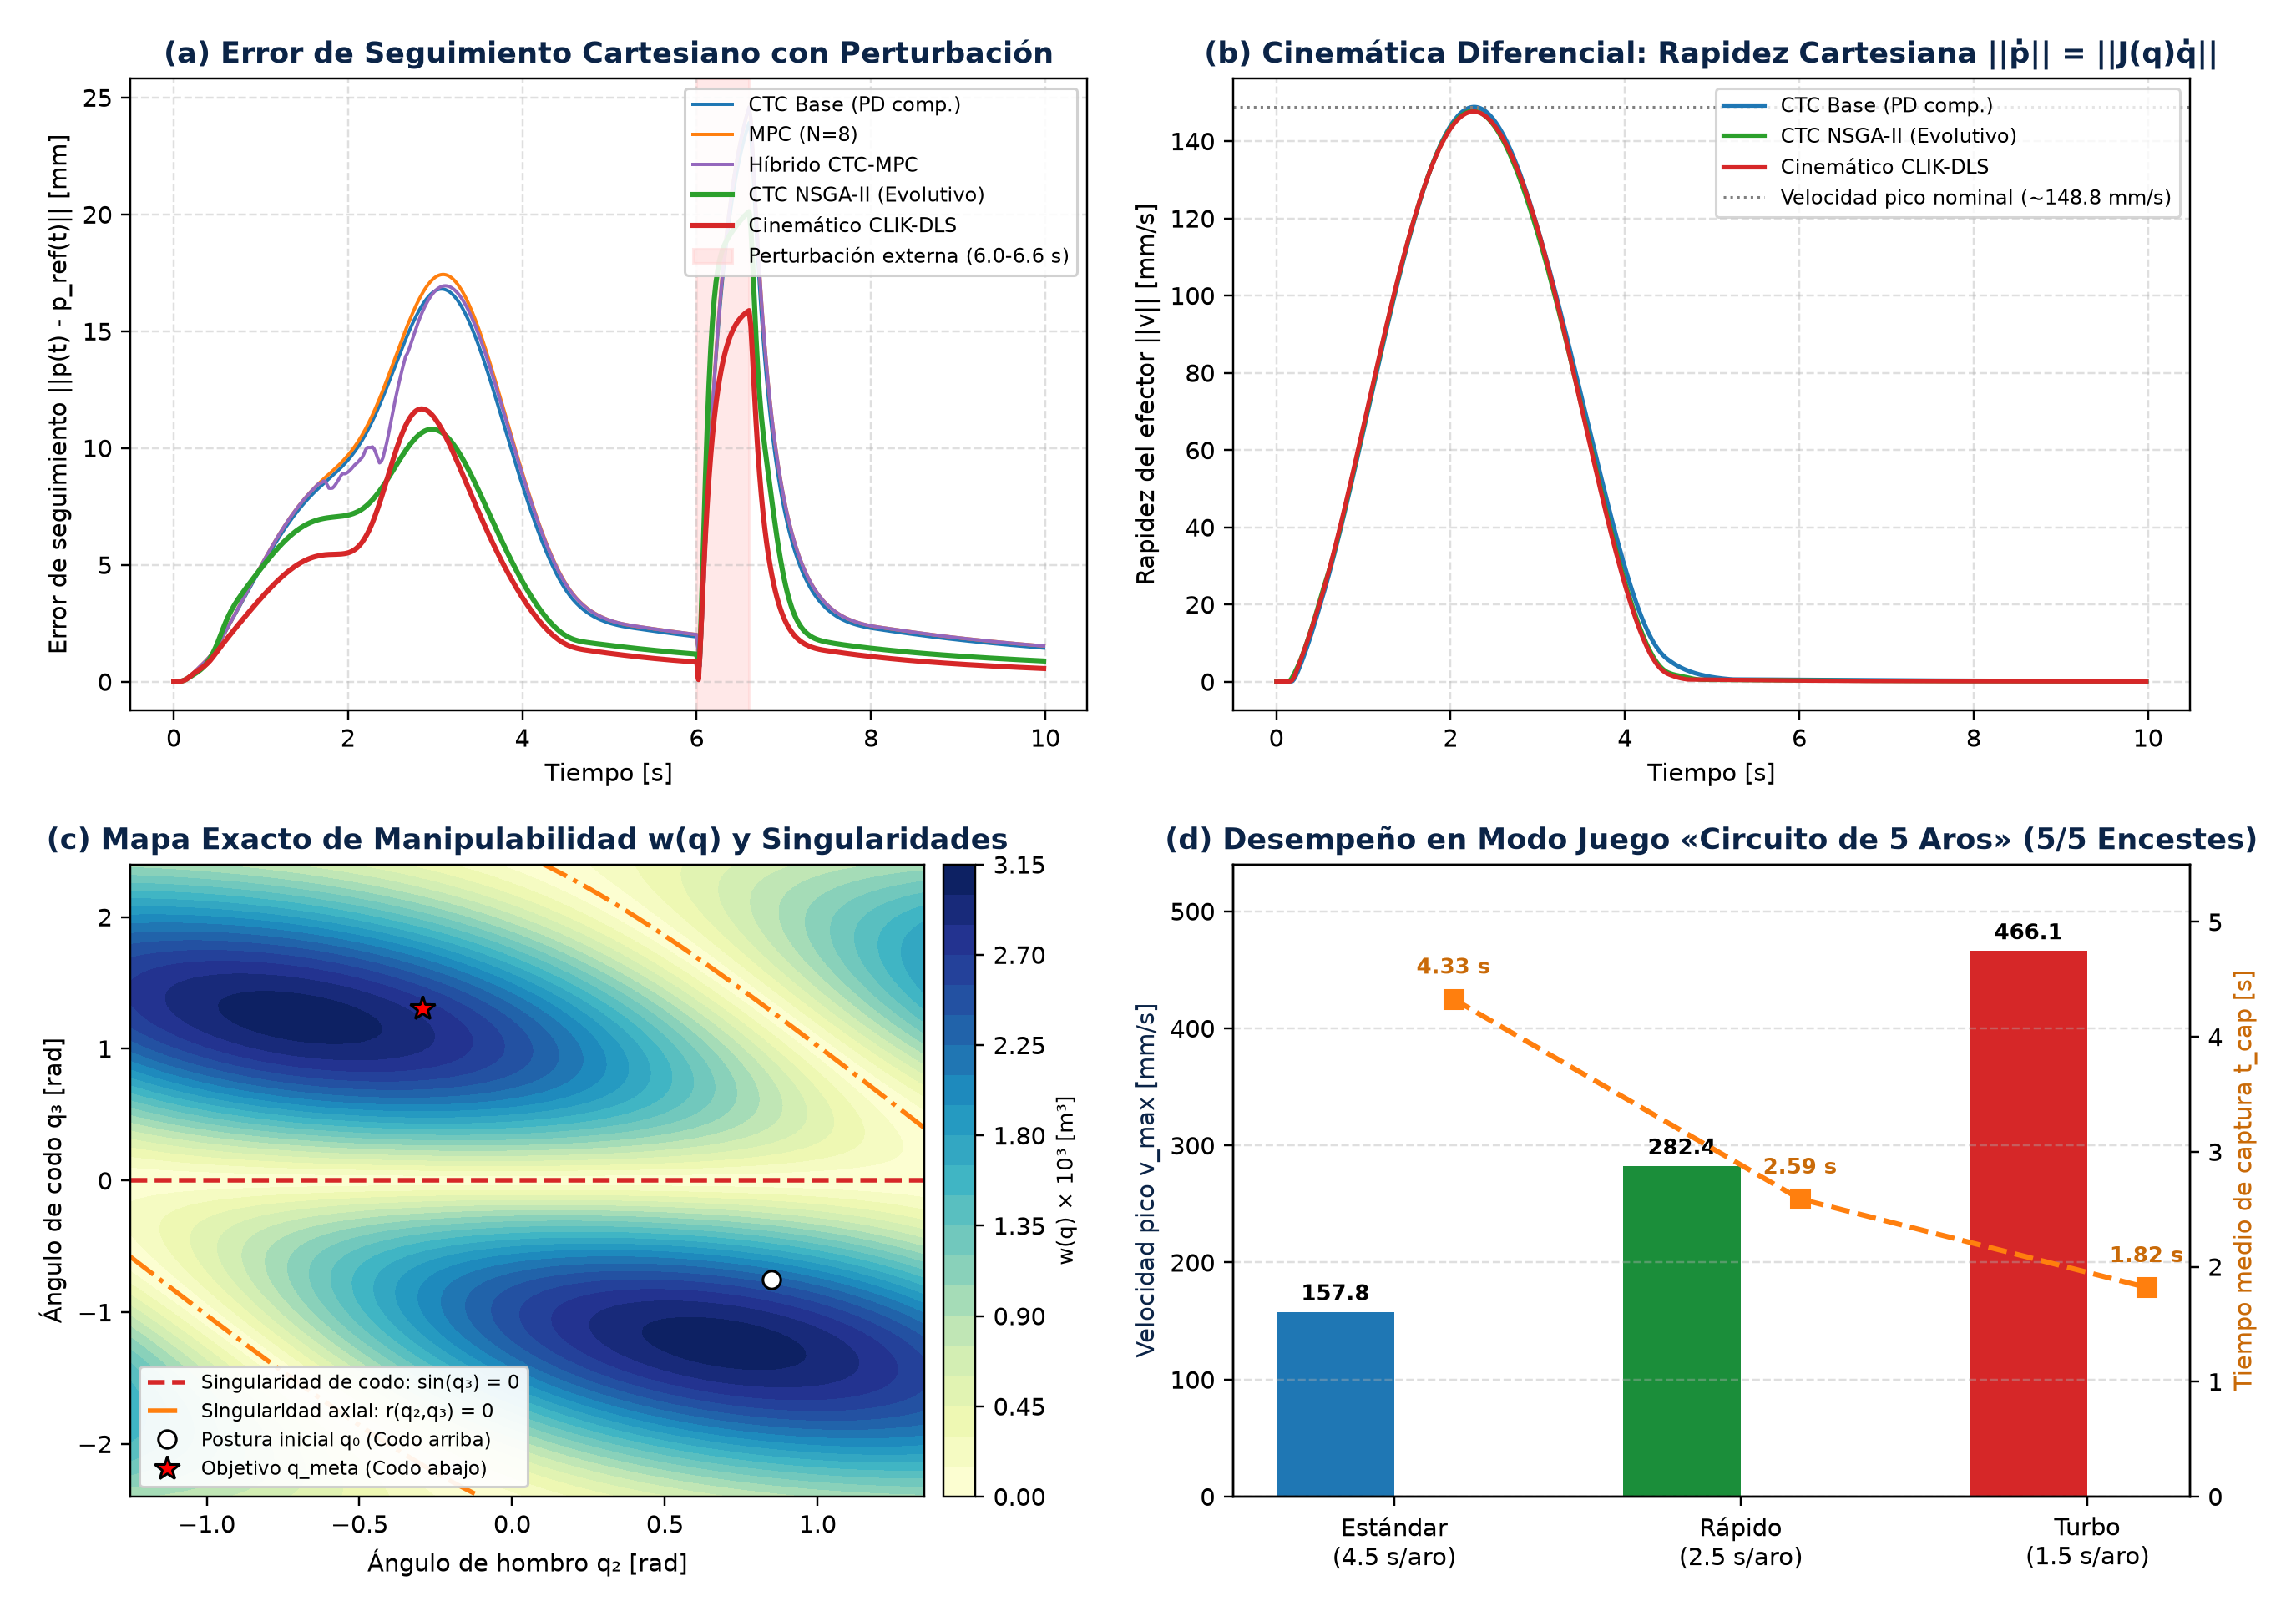
\includegraphics[width=0.98\linewidth,height=5.55cm,keepaspectratio]{results/figuras_examen_parcial/fig_curvas_simulacion.png}
    \end{cajadef}
  \end{column}

  \begin{column}{0.33\textwidth}
    \begin{cajaidea}[Lectura Milimétrica de los 4 Paneles]
      \fontsize{6.3}{7.6}\selectfont
      \begin{itemize}\setlength{\itemsep}{1.2pt}
        \item \textbf{Panel (a) Error Cartesiano:} Ante el pulso perturbador en $t\in[6{,}0,\,6{,}6]\;\text{s}$, \textbf{CLIK-DLS} (rojo) y \textbf{CTC NSGA-II} (verde) atenúan el pico y retornan a $<2\;\text{mm}$ en $0{,}242\;\text{s}$ y $0{,}382\;\text{s}$.
        \item \textbf{Panel (b) Rapidez $\norm{\pdot}$:} Campana suave sin discontinuidades gracias al interpolador quíntico $C^2$, con pico nominal de $148{,}8\;\text{mm/s}$.
        \item \textbf{Panel (c) Mapa Exacto $w(q_2,q_3)$:} Muestra la frontera de singularidad de codo ($\sin q_3 = 0$, línea roja) que el brazo cruza suavemente desde $\bm{q}_0$ (círculo blanco) hasta $\bm{q}_{\text{meta}}$ (estrella roja) vía DLS.
        \item \textbf{Panel (d) Perfiles de Juego:} Escalado de rapidez hasta $466{,}1\;\text{mm/s}$ en modo Turbo.
      \end{itemize}
    \end{cajaidea}
  \end{column}
\end{columns}
\end{frame}

% =====================================================================
% DIAPOSITIVA 11: MODO JUEGO «CIRCUITO DE 5 AROS» Y ESTADOS 3D
% =====================================================================
\begin{frame}{10. Aplicación Funcional: Modo Juego «Circuito de 5 Aros» y Estados 3D}{Transición Automática de Estado Visual en MuJoCo y Desempeño en Tres Perfiles de Rapidez}
\begin{cajadef}[Figura 3. Capturas Reales del Gemelo Digital 3D en MuJoCo (\texttt{main.py}): Máquina de Estados en Vivo]
  \centering
  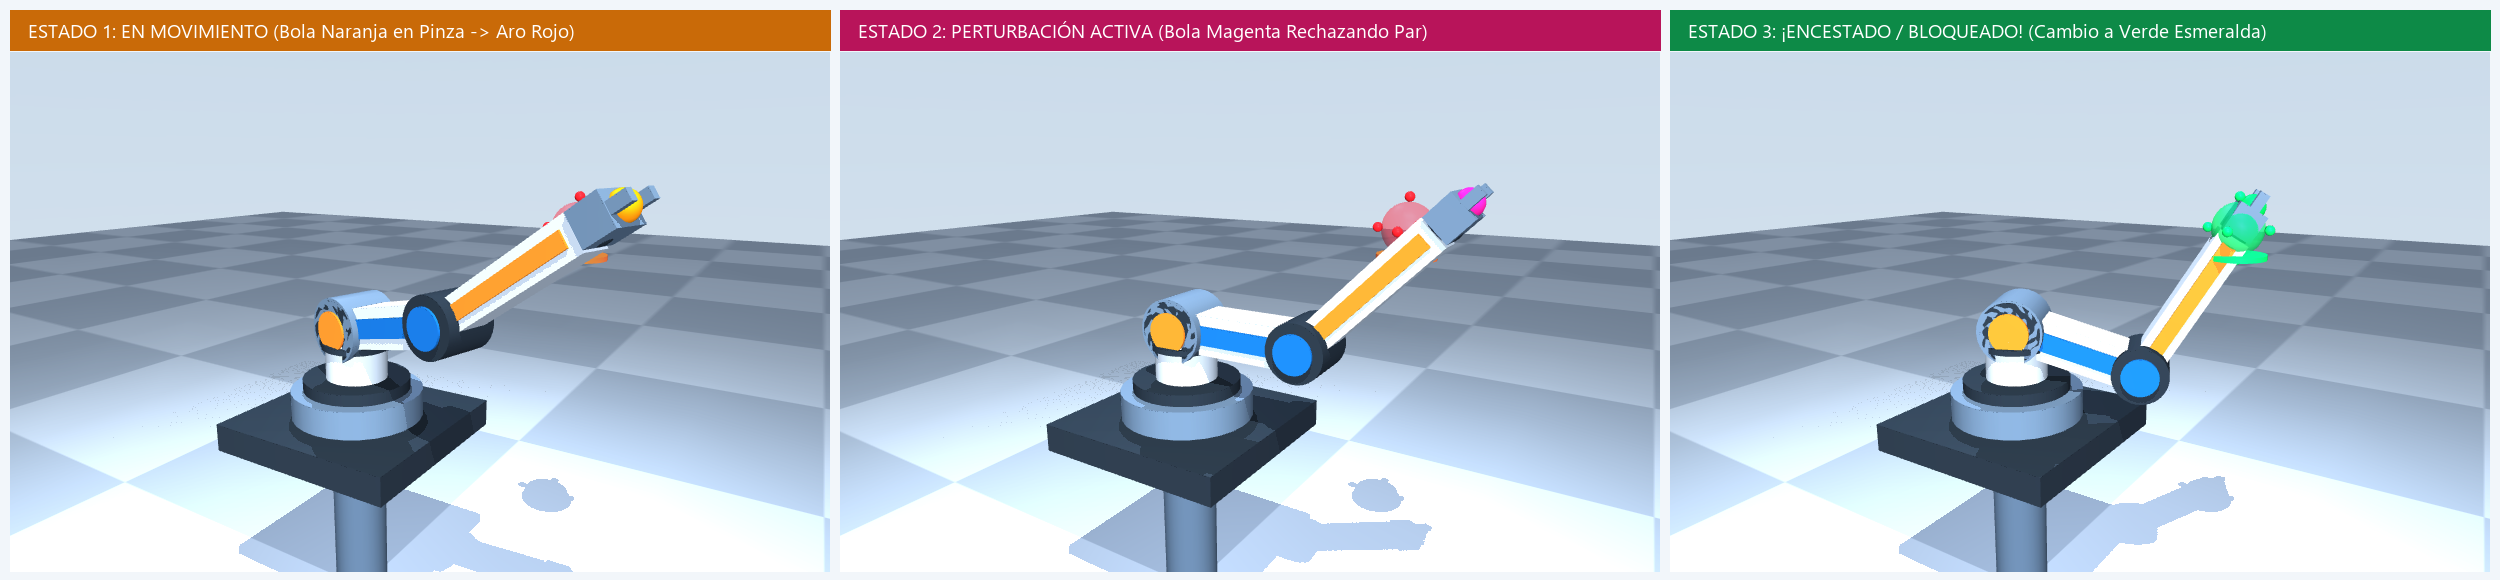
\includegraphics[width=0.90\linewidth,height=2.55cm,keepaspectratio]{results/figuras_examen_parcial/fig_estados_3d_enceste.png}\\[0.4mm]
  {\fontsize{5.8}{7.0}\selectfont\color{uniAzul}
  \textbf{Izquierda:} Estado 1 \emph{EN MOVIMIENTO} (esfera naranja $\to$ aro rojo) $\bullet$
  \textbf{Centro:} Estado 2 \emph{PERTURBACIÓN ACTIVA} (esfera magenta) $\bullet$
  \textbf{Derecha:} Estado 3 \emph{¡ENCESTADO!} (conmutan a \textbf{\color{verdeOk}Verde Esmeralda} cuando $\norm{\bm{p}(t)-\bm{p}_{\text{obj}}}<2{,}0\;\text{mm}$).}
\end{cajadef}

\vspace{0.5mm}
\begin{columns}[T,totalwidth=\textwidth]
  \begin{column}{0.58\textwidth}
    \begin{cajaidea}[Tabla 3. Métricas del Modo Juego «Circuito de 5 Aros»]
      \centering
      \resizebox{\linewidth}{!}{%
      \setlength{\tabcolsep}{3.8pt}
      \begin{tabular}{lcccccc}
        \toprule
        \textbf{Perfil} & \textbf{Dur./aro [s]} & \textbf{Encestes} & $t_{\text{cap}}$ \textbf{medio [s]} & $v_{\max}$ \textbf{pico [mm/s]} & \textbf{Rap. media [mm/s]} & \textbf{Energía [$\text{N}^2\text{m}^2\text{s}$]} \\
        \midrule
        Estándar & 4{,}5 & \textbf{5/5} & 4{,}33 & 157{,}8 &  52{,}5 & 1{,}1200 \\
        Rápido   & 2{,}5 & \textbf{5/5} & 2{,}59 & 282{,}4 &  87{,}0 & 0{,}6830 \\
        \rowcolor{green!10}
        Turbo    & 1{,}5 & \textbf{5/5} & \textbf{1{,}82} & \textbf{466{,}1} & \textbf{130{,}6} & \textbf{0{,}4670} \\
        \bottomrule
      \end{tabular}}
    \end{cajaidea}
  \end{column}

  \begin{column}{0.40\textwidth}
    \begin{cajaadv}[Verificación en Modo Turbo]
      \fontsize{6.2}{7.5}\selectfont
      El robot completa los \textbf{5/5 encestes} consecutivos alcanzando una rapidez pico de \textbf{$466{,}1\;\text{mm/s}$} y un tiempo medio de captura de \textbf{$1{,}82\;\text{s}$} por aro sin saturar el par de los actuadores Dynamixel.
    \end{cajaadv}
  \end{column}
\end{columns}
\end{frame}

% =====================================================================
% DIAPOSITIVA 12: CONCLUSIONES Y REFERENCIAS BIBLIOGRÁFICAS (APA 7)
% =====================================================================
\begin{frame}{11. Conclusiones Cuantitativas y Referencias Bibliográficas}{Síntesis de Hallazgos Científicos y Bibliografía en Norma APA 7.ª Edición}
\begin{columns}[T,totalwidth=\textwidth]
  \begin{column}{0.52\textwidth}
    \begin{cajaidea}[Conclusiones Principales del Trabajo Parcial]
      \fontsize{6.4}{7.7}\selectfont
      \begin{enumerate}\setlength{\itemsep}{1.0pt}
        \item \textbf{Equivalencia Cinemática Exacta:} Se demostró la identidad simbólica y numérica ($<10^{-15}\;\text{m}$) entre los métodos Geométrico, MTH y Denavit-Hartenberg en MATLAB y MuJoCo, y se resolvieron las dos ramas de cinemática inversa ($\sigma=\pm 1$) con error $\mathbf{0{,}00\;\text{mm}}$.
        \item \textbf{Cinemática Diferencial y Cruce de Singularidades:} Se formuló el Jacobiano geométrico completo $6\times 3$ ($J_v, J_\omega$) y se caracterizó $\det J_v = -L_1 L_2\sin(q_3)r(q_2,q_3)=0$, logrando cruzar la singularidad $\sin q_3=0$ sin picos de velocidad mediante $\Jdls(\bm{q})$ ($\lambda=0{,}018$).
        \item \textbf{Superioridad de CLIK-DLS y CTC NSGA-II:} \textbf{CLIK-DLS} alcanza el menor error final ($0{,}273\;\text{mm}$) y recuperación más rápida ($0{,}242\;\text{s}$); \textbf{CTC NSGA-II} reduce el RMSE en $33{,}5\,\%$ y el error estacionario en $42{,}2\,\%$ respecto al CTC base con menor energía ($0{,}4817\;\text{N}^2\text{m}^2\text{s}$).
        \item \textbf{Aplicación Funcional Interactiva:} El modo «Circuito de 5 Aros» logra \textbf{5/5 encestes} con cambio de estado visual 3D y rapidez pico de $466{,}1\;\text{mm/s}$.
      \end{enumerate}
    \end{cajaidea}
  \end{column}

  \begin{column}{0.46\textwidth}
    \begin{cajadef}[Referencias Bibliográficas (Norma APA 7.ª ed.)]
      \fontsize{5.3}{6.3}\selectfont
      \begin{itemize}\setlength{\itemsep}{0.5pt}
        \item Barrientos, A., Peñín, L. F., Balaguer, C., \& Aracil, R. (2007). \emph{Fundamentos de robótica} (2.ª ed.). McGraw-Hill.
        \item Buss, S. R. (2004). Introduction to inverse kinematics with Jacobian transpose, pseudoinverse and damped least squares methods. \emph{IEEE Journal of Robotics and Automation}, 17(1), 1--19.
        \item Conejo Benítez, C. E. (2021). \emph{Diseño e implementación de un brazo robótico antropomórfico de 3 grados de libertad para clasificación de objetos} [Trabajo de titulación, Univ.\ Politécnica Salesiana].
        \item Craig, J. J. (2018). \emph{Introduction to robotics: Mechanics and control} (4th ed.). Pearson.
        \item Deb, K., Pratap, A., Agarwal, S., \& Meyarivan, T. (2002). A fast and elitist multiobjective genetic algorithm: NSGA-II. \emph{IEEE Trans. Evol. Comput.}, 6(2), 182--197.
        \item Denavit, J., \& Hartenberg, R. S. (1955). A kinematic notation for lower-pair mechanisms based on matrices. \emph{Journal of Applied Mechanics}, 22(2), 215--221.
        \item Siciliano, B., Sciavicco, L., Villani, L., \& Oriolo, G. (2009). \emph{Robotics: Modelling, planning and control}. Springer.
        \item Todorov, E., Erez, T., \& Tassa, Y. (2012). MuJoCo: A physics engine for model-based control. \emph{IEEE/RSJ IROS}, 5026--5033.
        \item Yoshikawa, T. (1985). Manipulability of robotic mechanisms. \emph{The International Journal of Robotics Research}, 4(2), 3--9.
      \end{itemize}
    \end{cajadef}
  \end{column}
\end{columns}
\end{frame}

\end{document}